%%%%%%%%%%%%%%%%%%%%%%%%%%%%%%%%%%%%%%%%%%%%%%%%%%%%%%%%%%%%%%%%%%%%%%%%%%%%%%%
%% Electrochemical OER Application
%%
%% TODO: Put (s) on a-IrO3 phase in bulk Pourbaix diagram
%%%%%%%%%%%%%%%%%%%%%%%%%%%%%%%%%%%%%%%%%%%%%%%%%%%%%%%%%%%%%%%%%%%%%%%%%%%%%%%


% ################################# Paragraph #################################
% %%%%%%%%%%%%%%%%%%%%%%%%%%%%%%%%%%%%%%%%%%%%%%%%%%%%%%%%%%%%%%%%%%%%%%%%%%%%%
% Short introduction into the cataylsis section
% %%%%%%%%%%%%%%%%%%%%%%%%%%%%%%%%%%%%%%%%%%%%%%%%%%%%%%%%%%%%%%%%%%%%%%%%%%%%%
% | - Paragraph start
We next performed an {\it ab-initio} thermodynamic to elucidate the electrochemical operartional stability of IrOx
and OER activity of the four stable polymorphs (\rIrOtwo, \aIrOthree, \rIrOthree, and \bIrOthree) computed above (Fg. XYZ).


\subsubsection{Bulk Pourbaix}

% ################################# Paragraph #################################
% %%%%%%%%%%%%%%%%%%%%%%%%%%%%%%%%%%%%%%%%%%%%%%%%%%%%%%%%%%%%%%%%%%%%%%%%%%%%%
% Explain the Ir and IrO[4-] species
% #QUESTION Use E or U for potential variable
% %%%%%%%%%%%%%%%%%%%%%%%%%%%%%%%%%%%%%%%%%%%%%%%%%%%%%%%%%%%%%%%%%%%%%%%%%%%%%
% | - Paragraph start
Fig. \ref{fig:bulk_pourbaix} reports the IrOx pourbaix diagram (E vs. pH) constructed with the following species: Ir, \rIrOtwo, \aIrOthree,  \rIrOthree, \bIrOthree, and an aqueous dissolved \ce{IrO[4-]} species (See TEMP|SI for additional details).
%
While \Ir and \rIrOtwo are most stable at low bias, \aIrOthree is the most stable species under acidic conditions (pH \textless 7) and in the bias region of interest for the OER (~1.23 V vs. RHE).
%
% Raul | I would like to make the more general point that IrO3 polymorphs are the stable species relative to IrO2 at OER conditions.
% I think that point needs to be made clearly before we dive into the detail of which particular polymorph is stable
% TEXT | This indicates that the \aIrOthree phase may be stabilized under the highly oxidizing conditions of the OER.
%
% I want to be careful about how I talk about the metastable structures in the bulk Pourbaix, they strictly speaking shouldn't be there at all
The stability regions of the metastable \rIrOthree and \bIrOthree phases are indicated by unfilled solid lines and appear (meta?)stable in the OER relevant region of the diagram.
%
The similar formation energies (SI XYZ) for all three IrO3 species suggest some or all of these \ce{IrO_3} phases may be present and are stable under OER conditions.

% | - __old__
% , in the absence of any other competing \ce{IrO_3} polymorphs, are indicated by unfilled solid lines.
%
% As shown, these metastable phases appear to also have a wide region of stability in the OER region,
%due to to their formation energies being within TEMP eV of the globally stable \aIrOthree phase, see SI table TEMP for the bulk energies of all considered phases.
%
%Because of their similar energies it is possible that some or all of these \ce{IrO_3} phases may be present and relevant for the OER.
%
%In the next section, we explore this possibility by computing the theoretical OER activity of these polymorph systems.
% __|


% | - Figure | Bulk Pourbaix Diagram
\begin{figure*}[!htb]
\centering
\makebox[\textwidth][c]{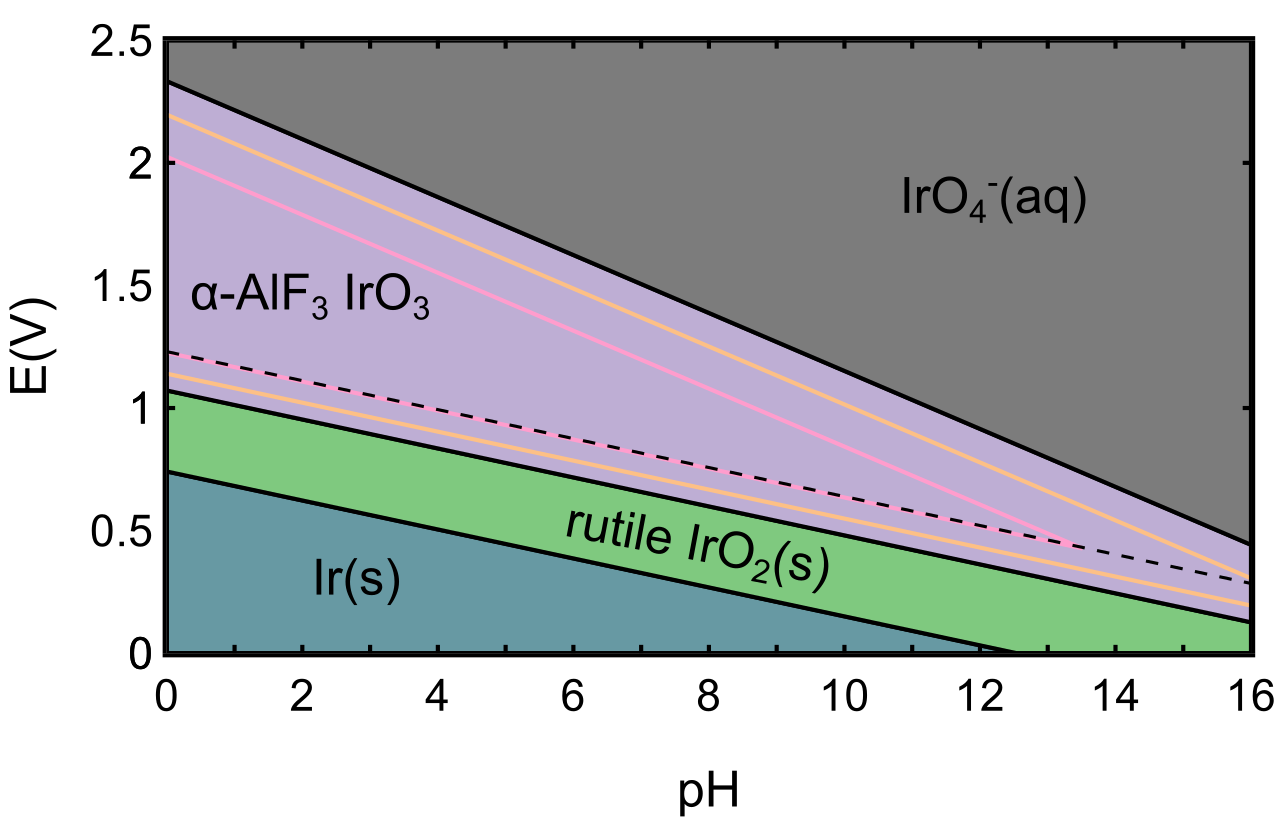
\includegraphics
{02_figures/oer_activity_stability/00_master__bulk-pourbaix__v1__400dpi__0__outplot.png}
% {02_figures/oer_activity_stability/bulk_pourbaix_0.pdf}
}
\label{fig:bulk_pourbaix}
\caption{
The revised Pourbaix diagram (electrochemical bulk phase stability)  of the Ir-H$_2$O system as a function of applied potential (vs. SHE) and pH. The most stable system studied (see Table XX in SI for a full list) are Ir-metal Ir(s) (blue), a \rIrOtwo  (green), and a dissolved \ce{IrO4[4-]} (gray). Thee are compared to the\ce{IrO_3} polymorphs, \aIrOthree (purple), \rIrOthree (orange), and \bIrOthree (pink). {\bf I would like to add Srx IrO3 to show much less stable it is than alpha}. The water equilibrium line at U=1.23 V vs RHE shows the ideal onset of OER. This plot highlights the importance of the \ce{IrO3} for OER operational stabity.
}
\end{figure*}
% __|

% __|

% __|


% | - OER Surfaces and Activities
\subsubsection{b. OER Surfaces and Activities}

% ################################# Paragraph #################################
% %%%%%%%%%%%%%%%%%%%%%%%%%%%%%%%%%%%%%%%%%%%%%%%%%%%%%%%%%%%%%%%%%%%%%%%%%%%%%
% Introduction to OER results
% %%%%%%%%%%%%%%%%%%%%%%%%%%%%%%%%%%%%%%%%%%%%%%%%%%%%%%%%%%%%%%%%%%%%%%%%%%%%%
Fig. \ref{fig:oer_volcano} summarizes the \sout{major} results of the electrochemical activity and surface stability analysis, structure files and method details are reported in SI XYZ.
%
Fig. \ref{fig:oer_volcano} a.) reports the surface energy Pourbaix plots as a function of applied potential (at pH=0) for the four IrOx crystals of interest.
%
The bulk phase limits of stability from figure TEMP are included at the bottom of each subplot.
%
For each polymoph, XYZ specific facets were chosen from the highest intensity x-ray diffraction peaks from powder-diffraction spectra simulated in VESTA (TEMP insert vesta ref and ref SI xrd plot) and physical intuition.
%
For each facet we computed the surface free energy for three coverages, bare, *OH, and *O.
% How facets were chosen | TODO Get x-ray pattern for systems
% TODO #REF | Reference for VESTA x-ray diff. pattern method
% TODO Say that the IrO3 bulk phase corresponds to the o-covered regime
%
% Probably remove this sentence and just go with the second one
% In most cases\chris{be specific}, the oxygen covered surfaces dominate at the OER equilibrium potential (1.23 V vs RHE) with bare surfaces being competitive to within TEMP eV/A2,
% this competitiveness goes away at even modest overpotentials (eta~0.3, --> ~1.5 V vs RHE),
% at which point the oxygen covered terminations are further over-stabilized relative to the bare surfaces,
% making them the sole dominant termination. Consequently, we consider mainly \chris{only?} oxygen terminated surfaces for the OER.\\
At modest overpotentials (eta ~0.3 and potentials of ~1.5 V vs RHE) the convex hull is populated solely by oxygen terminated surfaces.
%
% COMBAK, Revise "mainly" if we include some different coverages
Consequently, we consider mainly oxygen terminated surfaces for the OER analysis.
%
% __|

% ################################# Paragraph #################################
% %%%%%%%%%%%%%%%%%%%%%%%%%%%%%%%%%%%%%%%%%%%%%%%%%%%%%%%%%%%%%%%%%%%%%%%%%%%%%
% OER results
% %%%%%%%%%%%%%%%%%%%%%%%%%%%%%%%%%%%%%%%%%%%%%%%%%%%%%%%%%%%%%%%%%%%%%%%%%%%%%
% | - Paragraph start
% Replace G_O and G_OH with my custom macros for consistency
The OER activity (expressed in terms of the limiting potential) for select oxygen terminated surfaces are shown in Fig. \ref{fig:oer_volcano} as a function of the $\Delta G_\mathrm{O} - \Delta G_\mathrm{OH}$ thermodynamic descriptor.
%
The two rutile-IrO2 surfaces (100 and 110) bind the OER intermediates strongly, locating them at a theoretical limiting potential of xyz.
%
The predicted overpotentials of our rutile-IrO2 systems are within the range of experimentally observed overpotentials found in literature.
% Reference all experimental IrO2 overpotentials I can find
%
The three IrO3 polymorph surfaces all have a $\Delta G_\mathrm{O} - \Delta G_\mathrm{OH}$ descriptor towards the top and right of the volcano, indicative of weaker binding energetics.
% \chris{Im losing the big picture here at the end of the section, I think you are convoluting two different things that need to be broken up into their own paragraphs.  This OER activity part needs some work, let's discuss}
%
This is evident from figure SI TEMP (scaling) which shows a clear distinction between the IrO2 and IrO3 polymorphs, with IrO3 binding on average TEMP eV weaker than IrO2.
%
The best performing systems, including the (100), (110), and (211) facets of a-IrO3, b-IrO3 (101), and R-IrO3 (110), have overpotentials of ~0.4 V vs RHE,
a ~0.2 V vs RHE improvement over the rutile-IrO2 system.
%
We note that the computed  overpotentials for our \rIrOtwo system differs from that reported in \cite{Seitz2016} by ~0.2 V. This discrepancy is due to our us of spin-polarization, which was neglected in Seitz et al., which strengthens the binding of IrO2.

% | - Figure | OER Volcano/Surface Pourbaix
\begin{figure*}
\centering
\makebox[\textwidth][c]{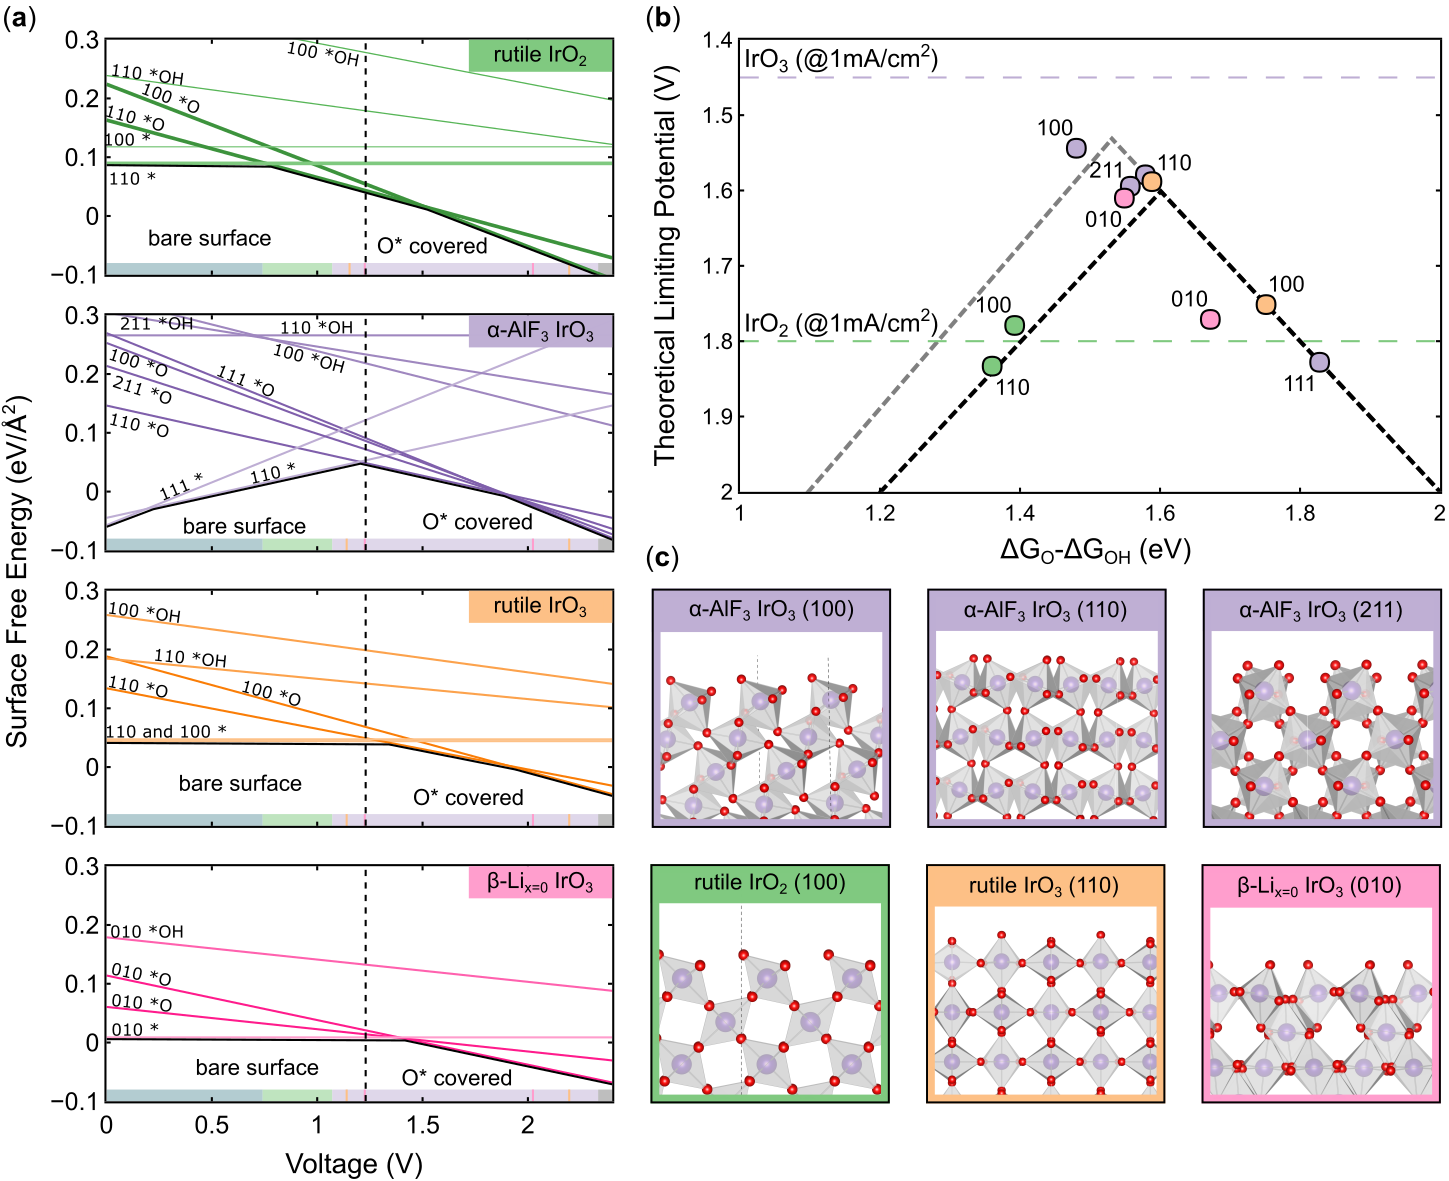
\includegraphics
{02_figures/oer_activity_stability/00_master__oer-volc_surf-pourb_struct__main_v3__200dpi__outplot.png}
% {02_figures/oer_activity_stability/00_master_plot__oer-volc_surf-pourb_struct__main_v3__outplot.pdf}
}
\caption{\label{fig:oer_volcano}
Summary of OER results for the four bulk structures of \IrOx considered: rutile-\ce{IrO_2} (green), $\alpha$-\ce{IrO_3} (purple), rutile-\ce{IrO_3} (orange), and $\beta$-\ce{IrO_3} (pink).
%
(a) Surface energy Pourbaix diagrams for each structure, with the surface energy of various facets and coverages shown as a function of applied potential.
The bulk Pourbaix diagram's bounds of stability at pH 0 are superimposed at the bottom of each subplot.
%
(b) OER activity volcano for \IrOx systems considered utilizing the \DGOmOH thermodynamic descriptor.
The purple dotted line corresponds to the experimental limiting potential at 10 mA cm\textsuperscript{2} for \ce{IrO_3} \cite{Seitz2016},
while the green band corresponds to the range of experimentally observed overpotentials for pristine \ce{IrO_2} catalysts as reported in literature.  % TODO Insert green band into figure, insert experimental references for this
%
(c) Select surface facets for the four \IrOx crystal systems considered.
%
% | - __old__
% Circles designate oxygen covered surfaces while triangles designate hydroxyl (*OH) terminated surfaces (relevant surface terminations were found via surface Pourbaix analyses).
% Surface energies at standard conditions (pH and V = 0) are reflected in the border color for each data point, where black indicates a low energy surface termination and white indicates more unstable surfaces.  % Currently not implemented as this
% The color range goes from x to y.
% __|
}
\end{figure*}
% __|

% __|


% | - OER Scaling Relations | TODO | MOVE THIS TO SI
\subsubsection{c. OER Intermediate Scaling}
{\bf We will make a O(2p) vs O-OH plot showing that this descriptor correlates with oxidation state like that some of the structures are close to ideal.}

% ################################# Paragraph #################################
% %%%%%%%%%%%%%%%%%%%%%%%%%%%%%%%%%%%%%%%%%%%%%%%%%%%%%%%%%%%%%%%%%%%%%%%%%%%%%
% TEMP
% %%%%%%%%%%%%%%%%%%%%%%%%%%%%%%%%%%%%%%%%%%%%%%%%%%%%%%%%%%%%%%%%%%%%%%%%%%%%%
Figure TEMP shows the scaling relations between the adsorption free energies of the OER intermediate species for the \IrOx systems studied herein.
%
It can be seen clearly that the data points corresponding to the three \ce{IrO_3} polymorphs are roughly 1 eV weaker binding than the rutile-\ce{IrO_2} points.
%
This generally weaker binding of the \ce{IrO_3} stoichiometry is responsible for the observed improvement in theoretical activity.
%
The \DGOOH vs.\DGOH relationship is very close to the traditional ``universal scaling relations'', demonstrating that our materials do not break the infamous \DGOOH vs. \DGOH scaling.


% | - Figure | OER Scaling Relations
\begin{figure*}
\centering
\makebox[\textwidth][c]{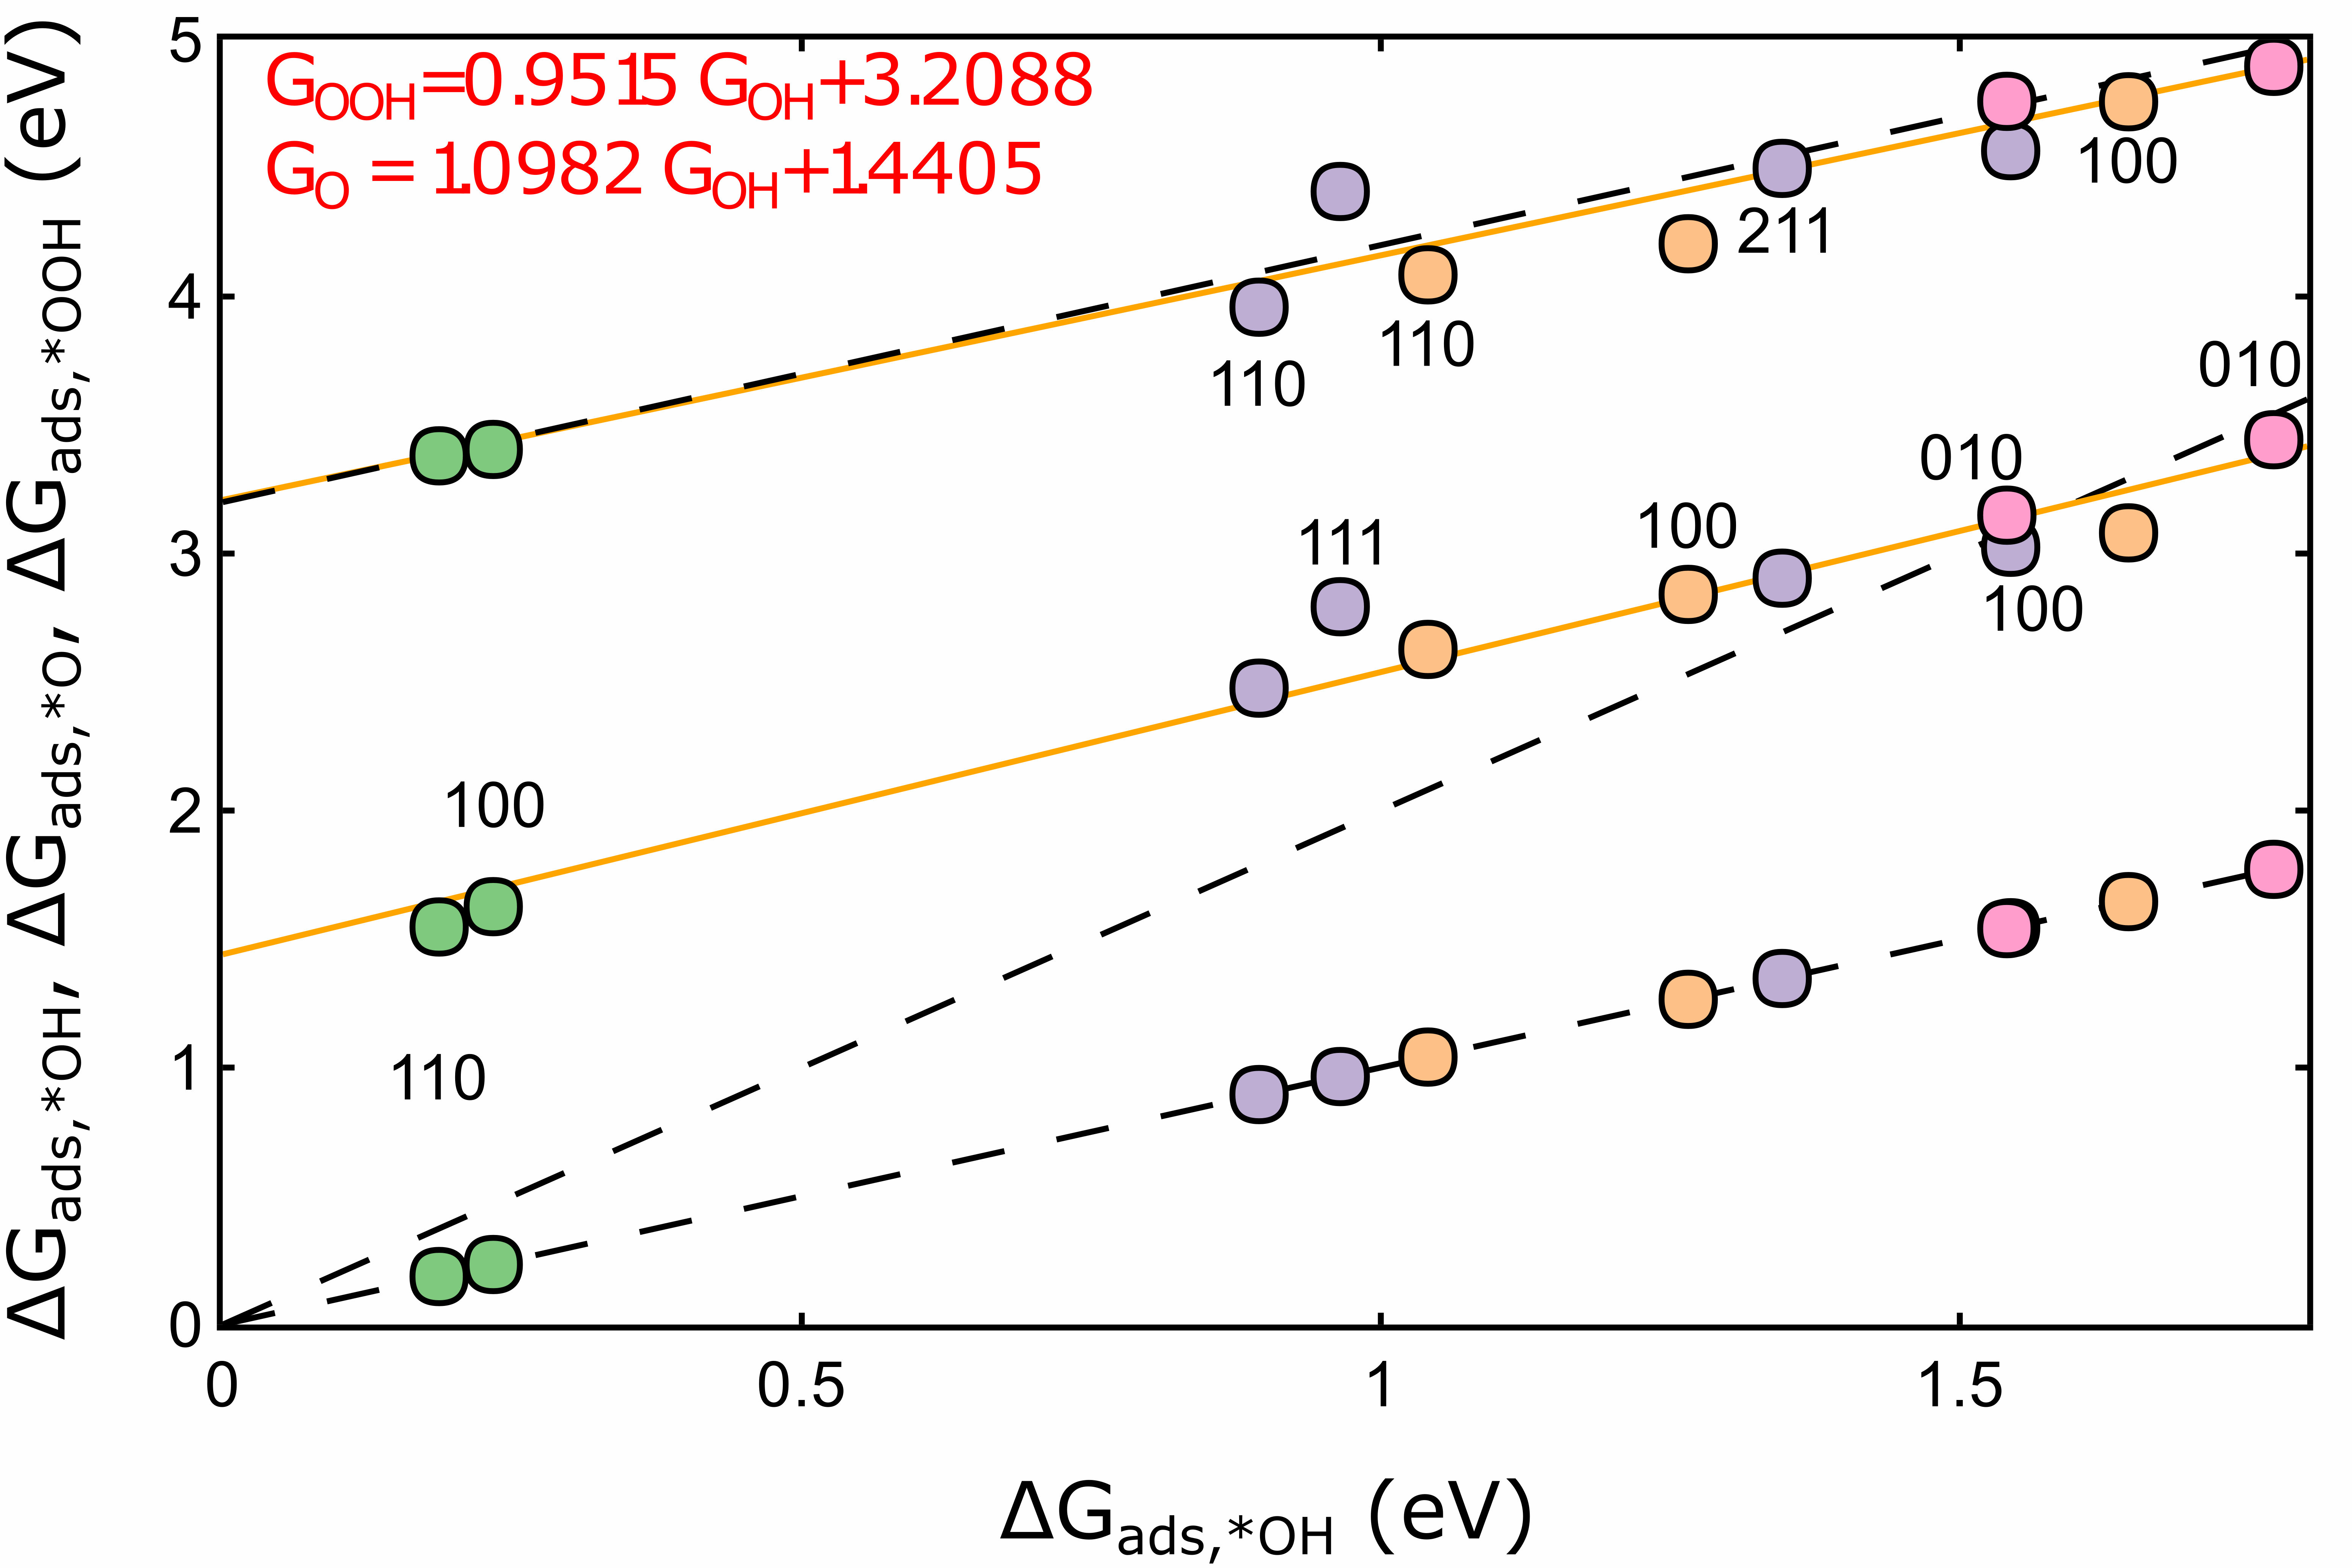
\includegraphics
{02_figures/oer_activity_stability/00_master__oer_scaling__main_v0__outplot2.png}
% {02_figures/oer_activity_stability/pl_scaling_relations_tmp.pdf}
}
\caption{\label{fig:scaling_relations}
% Adsorption free energy scaling relations plot.
Relationship between the adsorption free energies of the three key OER intermediates (*OH, *O, *OOH), with \DGOH chosen as the dependent variable.
Best fit lines are provided for \DGOOH vs. \DGOH and \DGO vs. \DGOH.
%
Additionally, ``universal scaling relations'' for \DGOOH vs. \DGOH and \DGO vs. \DGOH are shown (black dotted lines) to emphasize our deviation from the traditionally reported scaling fits.
The \DGOH line is  shown as guide to eye.
% TODO Do I have to redefine the color convention every caption?
}
\end{figure*}
% __|

% __|
